\documentclass{article}
\usepackage{tmlr}
% \usepackage[accepted]{tmlr}   % uncomment for the camera-ready
% \usepackage[preprint]{tmlr}   % uncomment for a non-anonymous preprint

\usepackage{amsmath,amssymb,booktabs,graphicx,xcolor}
\usepackage{pgfplots}
\pgfplotsset{compat=1.18}
\usepgfplotslibrary{fillbetween}
\graphicspath{{../results/}}

\title{Is the Safety and Hallucination Feature Geometry of \\ Language Models Conditional on Dialogue Context? \\ A Confound-Controlled Study}

\author{\name Anonymous \email anon@example.com \\ \addr Affiliation withheld for review}

\def\month{06}
\def\year{2026}
\def\openreview{\url{https://openreview.net/forum?id=XXXXXXXXXX}}

\begin{document}
\maketitle

\begin{abstract}
A growing class of inference-time alignment methods, conditional activation
steering and conditional subspace disentanglement of hallucination from safety,
rests on an implicit premise: that the low-dimensional residual-stream directions
encoding safety/refusal and epistemic uncertainty are \emph{conditional} on dialogue
context, so that a single static intervention learned on one context is
mis-specified for another. We ask whether this premise is empirically true, and find
that the obvious ways of measuring it are confounded. We introduce a confound-controlled
protocol: subspaces are recovered by contrastive difference-of-means, drift is measured
as a gauge-invariant chordal distance between subspaces, and ``the subspace moved with
context'' is tested against (i) a turn-1 baseline that removes the generic
no-context$\to$context jump, (ii) a length- and topic-matched \emph{scrambled-twin}
null that holds token count and lexical content fixed while destroying coherent
meaning, and (iii) a dialogue-level bootstrap confidence interval so that no single
dialogue can carry the result. Applied to an instruction-tuned model, three intuitive
positive measurements (cumulative displacement, between-dialogue spread versus a
same-context floor, and a small-sample placebo comparison) are each overturned by the
next control. Under the full protocol, the apparent context-conditionality of the
hallucination subspace is statistically indistinguishable from a length/topic artifact:
scrambled twins move the subspace as much as real dialogues, and the real-versus-placebo
confidence intervals overlap at every layer. We further fit the static disentangling
projector these methods would replace and show its across-turn re-entanglement is fully
matched by the length/topic placebo, i.e.\ the static baseline does not genuinely fail. Beyond the specific null, the transferable
contributions are a reusable protocol, a taxonomy of three confounds that each
independently produce a false positive (a no-context onset, a same-context null that is
rigged to fire, and small-sample single-dialogue effects), and a control checklist for
anyone making a ``context changes the representation'' claim; we also derive an actionable
requirement for conditional-alignment methods, namely that they report this controlled
measurement before assuming the premise. We report the null as scoped to the models and
conditions tested. \textbf{All numbers in this draft are from
real runs on the released code. The null replicates across two model scales in raw
activation space (0.5B, 1.5B) and, critically, in sparse-autoencoder feature space (the
space disentanglement methods operate in), where the scrambled twin moves the subspace
\emph{more} than real dialogues at the late layers. The larger-instruction-model and
mixture-of-experts cells are in progress and are marked as such.}
\end{abstract}

\section{Introduction}
\label{sec:intro}

Mechanistic interpretability has established that high-level behaviors of large language
models (LLMs) are often approximately linearly encoded: refusal is mediated by a single
residual-stream direction \citep{arditi2024refusal}, truth/falsehood is linearly
represented \citep{marks2023geometry}, and sparse autoencoders (SAEs) recover
interpretable feature directions at scale \citep{bricken2023monosemanticity,
templeton2024scaling, lieberum2024gemmascope}. These directions can be read and steered
\citep{zou2023repe, li2023iti, panickssery2024caa} and erased in closed form
\citep{ravfogel2020inlp, belrose2023leace}.

A natural next step, pursued by recent work, is to \emph{disentangle} behaviors that
share latent components: for example, to mitigate hallucination without degrading safety
by orthogonalizing the SAE subspaces that encode them \citep{mahmoud2025unintended}. Once
one moves from a single static edit to a \emph{conditional} one, an implicit empirical
premise enters: that the relevant geometry is conditional on context, so that a single
projection learned on one context (or on single-turn data) is mis-specified elsewhere,
and in particular drifts as a multi-turn dialogue accumulates. This premise is rarely
stated, let alone tested. It is also non-obvious: the geometry-of-refusal literature has
shown that geometric orthogonality need not imply behavioral independence
\citep{wollschlager2025geometry}, that refusal is multi-directional \citep{pan2025hidden},
and that steering vectors generalize poorly and are brittle \citep{tan2024steering}.

We ask the prior question directly: \emph{does dialogue context actually rotate the
safety and hallucination subspaces, beyond trivial confounds?} The contribution is not a
new alignment method but a measurement and a caution:

\begin{itemize}
\item \textbf{A confound-controlled protocol} (\S\ref{sec:method}) for testing
representational drift: gauge-invariant chordal drift between contrastively-recovered
subspaces, a turn-1 baseline, a length/topic-matched scrambled-twin null, and
dialogue-level bootstrap confidence intervals. The protocol is validated against analytic
ground truth.
\item \textbf{A rigor cascade} (\S\ref{sec:cascade}) showing that three intuitive
positive measurements of context-conditionality are each artifacts: a no-context onset
jump, a same-context null that carries no length/topic variance, and a small-sample
($n{=}3$ dialogue) placebo comparison.
\item \textbf{A robustness finding} (\S\ref{sec:main}): under the full protocol the
hallucination subspace's apparent context-conditionality is statistically indistinguishable
from a length/topic artifact, and this null \emph{replicates} across two model scales in raw
activation space and in SAE feature space, the representation conditional disentanglement
actually uses; the safety/refusal subspace is not even cleanly recoverable below the mid
layers, so the targeted cross-subspace entanglement cannot be measured where it would be
needed.
\item \textbf{Actionable recommendations} (\S\ref{sec:lessons}): a control checklist for
representational-drift claims, and the requirement that conditional-alignment methods report
the controlled premise measurement (and a failing static baseline) before introducing
conditional machinery.
\end{itemize}

We frame this as a robustness/methodology study rather than a single negative number: the
generalizable output is the protocol, the confound taxonomy, and the recommendations, with
the replicated null as the evidence that they matter.

Our claim is deliberately scoped: we do not claim the premise is false for all models or
in SAE feature space. We claim that the premise is \emph{not supported} by the obvious
measurements once they are controlled, that the controls matter (they flip the
conclusion), and that methods built on this premise should report the controlled
measurement before assuming it.

\section{Related Work}
\label{sec:related}

\subsection{Linear representations, sparse features, and their skeptics}

A growing body of evidence supports the linear-representation view that high-level concepts are encoded as directions in the residual stream $x \in \mathbb{R}^d$, recoverable by linear probes and difference-of-means contrasts \citep{marks2023geometry}. Sparse autoencoders (SAEs) extend this picture by decomposing activations into an overcomplete dictionary of approximately monosemantic features \citep{bricken2023monosemanticity,cunningham2023sparse,templeton2024scaling}, and open suites now make such dictionaries available across layers and architectures \citep{lieberum2024gemmascope,gao2024scaling,rajamanoharan2024jumprelu}. Within this line, several latents have been linked to epistemic and knowledge-awareness behavior relevant to hallucination, for instance entity-recognition features that fire on known versus unknown entities \citep{ferrando2025entity}. Our hallucination/epistemic subspace $H_t$, contrasting answerable real-entity against surface-matched unanswerable fictional-entity questions, targets the same phenomenon, though we recover it by contrast at each dialogue turn rather than reading off a fixed dictionary. A parallel skeptical literature cautions that the interpretability value of these features is easy to overstate: SAE-derived probes can underperform simple baselines on downstream tasks \citep{kantamneni2025useful}, and common SAE proxy metrics do not reliably track the downstream quantities they are meant to predict \citep{karvonen2025saebench}. This tension, between features that look meaningful in isolation and features that earn their keep under controlled evaluation, motivates the measurement framing we adopt: a geometric signal that appears present must be shown to survive the right null before it is treated as real.

\subsection{Steering and concept erasure}

A complementary line treats these directions as handles for intervention rather than objects of study. Representation engineering reads and writes concept directions to control model behavior \citep{zou2023repe}, with task-specific instances including inference-time intervention for truthfulness \citep{li2023iti}, contrastive activation addition \citep{panickssery2024caa}, and the identification of a single refusal direction whose ablation via weight orthogonalization removes safety behavior \citep{arditi2024refusal}. The dual operation, removing a concept, is formalized by closed-form concept erasure \citep{belrose2023leace} and nullspace projection \citep{ravfogel2020inlp}. These methods presuppose that the relevant concept occupies a stable, low-dimensional subspace that an intervention can target. Our safety subspace $S_t$ (harmful versus surface-matched harmless requests) and the static disentangling projector we stress-test are built directly on this presupposition: the projector is fit once and asked to hold across turns. Whether such a static target is adequate, or whether it must be re-estimated as dialogue content changes, is precisely the question a conditional treatment of these subspaces raises.

\subsection{Conditional steering and conditional disentanglement}

The premise we test belongs to a recent and still thin line that makes intervention \emph{conditional} on dialogue content: the claim that the safety and hallucination geometry shifts with what has been said, so that a context-dependent (rather than static) subspace is needed to steer or to disentangle reliably. The closest method is \citet{mahmoud2025unintended}, which combines SAEs with subspace orthogonalization to disentangle hallucination from safety, with the goal of intervening on one without unintended effects on the other. This is the method whose premise our study evaluates: if the relevant subspaces drift with content, a static disentangler should leak as context accumulates, motivating a conditional one. We emphasize that this is a single recent preprint, so the conditional-disentanglement hypothesis is best regarded as an open conjecture rather than an established regularity, and our contribution is to ask whether its motivating premise holds under confound control on the models we evaluate, rather than to propose a competing intervention.

\subsection{Brittleness of steering and the geometry of refusal}

Several results already complicate any simple static-versus-conditional dichotomy, from both directions. On one side, steering vectors are reported to be brittle and to generalize poorly out of distribution \citep{tan2024steering}, which could be read as evidence that a static direction is insufficient and that conditioning on context is required. On the other side, the refusal direction is not as singular as the one-direction picture suggests: refusal appears to be multi-directional \citep{pan2025hidden}, and concept representations form cones in which geometric orthogonality between two concepts does not imply that interventions on them are independent \citep{wollschlager2025geometry}. These findings matter for our measurement because they decouple two things that a naive reading conflates. Apparent failure of a static subspace, or apparent movement of one, need not be content-conditionality: it can instead reflect multi-directional structure, cone geometry, or the gauge freedom in choosing an orthonormal basis $U_t$. We therefore work with gauge-invariant quantities throughout, the chordal drift $d(U,V) = \sqrt{\operatorname{mean}_i \sin^2 \theta_i}$ and the cross-overlap $\Omega(S_t,H_t) = \lVert U_S^\top U_H \rVert_F^2 / k$ defined via principal angles \citep{edelman1998geometry}, so that a reported drift cannot be an artifact of how the bases were oriented. The lesson we draw from this literature is that brittleness and apparent drift are necessary but not sufficient evidence for content-conditionality, and that distinguishing a genuine content effect from a confound requires an explicit null.

\subsection{Measurement, confound control, and our contribution}

Where prior work largely assumes a representational structure and then intervenes on it, we treat the structure itself as the object of measurement and ask whether a specific structural claim, content-conditionality of $H_t$ and $S_t$, survives controls. The central methodological point is the choice of null. The naive null, two bootstrap resamples of the same probe set at a fixed context, carries zero between-condition length and topic variance, so on a between-context statistic the comparison ``spread exceeds floor'' is near-tautological. We instead require that genuine content-conditionality exceed a scrambled-twin null that word-shuffles each user turn, preserving the exact token multiset (length, topic, and lexicon) while destroying coherent meaning, with dialogue-level bootstrap confidence intervals so the verdict does not rest on a single dialogue. This protocol isolates three confounds, the no-context probe-in-context onset, token length and final-token position, and single-dialogue idiosyncrasy, and we show that each, left uncontrolled, manufactures a positive result that the next control overturns. Validated against analytic ground truth (a recovered $15^\circ$/turn injected rotation, and a static subspace correctly returning drift at the bootstrap floor) and powered through a reported noise floor, the protocol returns \texttt{NOT\_CONTENT\_CONDITIONAL} on every setting we evaluate: Qwen2.5-0.5B-Instruct and Qwen2.5-1.5B-Instruct \citep{qwen25} in raw activations, and GPT-2 small in the SAE feature space of residual SAEs, the space these methods actually use. A static disentangling projector that appears to fail across turns leaks no more than its length and topic scrambled twin, so its apparent failure is a confound rather than evidence that a content-conditional projector is needed. Our scope is deliberately bounded to these instruction-tuned and GPT-2 models and to rank-1 difference-of-means subspaces; against benchmarks such as TruthfulQA \citep{lin2022truthfulqa} and over-refusal probes like XSTest \citep{rottger2024xstest} that drive much of the steering literature, the contribution here is not a new direction or a new intervention but a reusable, pre-registered protocol and a set of controls that let future work tell a real content effect apart from a length and topic artifact before building conditional machinery on top of it.

\section{Method}
\label{sec:method}

We study a single, precise question: does dialogue context rotate the low-dimensional
residual-stream subspaces that encode hallucination/epistemic state and safety/refusal,
beyond what is explained by trivial nuisance variables (prompt length, final-token
position, and surface topic)? This section defines the estimator, the gauge-invariant
drift metric, the projector-leak identity that operationalizes ``a static intervention is
mis-specified,'' the three confounds and their controls, and the pre-registered decision
rule. Throughout, a residual activation is $x \in \mathbb{R}^d$, read at the last token of
a prompt at a fixed layer.

\subsection{Subspace estimation by contrast}
\label{sec:subspace}

At dialogue turn $t$ we form a prompt by prepending the running conversation (the first
$t$ user turns, each followed by a fixed, neutral assistant reply that carries no
task-relevant content) and appending a held-out contrastive probe as the next user turn.
The conversation context is the \emph{only} thing that varies across turns: the probe bank
is fixed across all turns and all dialogues, so any movement we measure in the recovered
subspace is attributable to the prepended context rather than to a change of probes.

We recover concept subspaces by contrastive difference-of-means, the standard construction
behind linear probing and steering directions
\citep{marks2023geometry, arditi2024refusal, panickssery2024caa}. For the
\emph{hallucination/epistemic} subspace $H_t$ we use answerable real-entity questions
paired with surface-matched unanswerable fictional-entity questions, the
knowledge-awareness contrast of \citet{ferrando2025entity}; for the \emph{safety} subspace
$S_t$ we use harmful requests paired with surface-matched harmless requests, the refusal
contrast of \citet{arditi2024refusal}. Let $\{(x_i^{+}, x_i^{-})\}_{i=1}^{n}$ be the
last-token activations of the $n$ matched pairs at turn $t$, and let
$\delta_i = x_i^{+} - x_i^{-}$ be the per-pair difference vectors. Stacking the (centered)
$\delta_i$ into $D \in \mathbb{R}^{n \times d}$, we take $U_t \in \mathbb{R}^{d \times k}$
to be an orthonormal basis for the top-$k$ right singular vectors of $D$ (equivalently the
top-$k$ eigenvectors of $\sum_i \delta_i \delta_i^\top$). The default is the rank-1
difference-of-means direction, $k=1$, normalized to unit length;
Section~\ref{sec:power} explains why higher rank is not usable at our probe budgets. Pairing
removes the content the two sides share by construction, so $U_t$ isolates the concept axis
(epistemic status, or harmfulness) rather than the surface form of the probe.

\subsection{Gauge-invariant chordal drift}
\label{sec:drift}

A difference-of-means subspace is recovered only up to an arbitrary orthonormal basis: the
estimator returns \emph{a} basis $U_t$ for the plane $\mathrm{span}(U_t)$, and any
$U_t R$ with $R \in O(k)$ spans the same plane. A drift metric must therefore be a
function of the planes, not of the bases. Given two $k$-planes with orthonormal bases
$U, V \in \mathbb{R}^{d \times k}$, let $\theta_1, \dots, \theta_k$ be their principal
angles, defined through the singular values $\sigma_i = \cos\theta_i$ of $U^\top V$
\citep{edelman1998geometry}. We measure drift by the normalized chordal distance
\begin{equation}
\label{eq:chordal}
d(U, V) \;=\; \sqrt{\frac{1}{k} \sum_{i=1}^{k} \sin^2 \theta_i} \;\in\; [0, 1],
\end{equation}
which is $0$ when the planes coincide ($\theta_i = 0$ for all $i$) and $1$ when they are
orthogonal ($\theta_i = \pi/2$).

\paragraph{Derivation of the projector form and basis-invariance.} The quantity in
\eqref{eq:chordal} equals a Frobenius distance between the two orthogonal projectors
$P_U = U U^\top$ and $P_V = V V^\top$, which makes its basis-invariance manifest. Using
$\|A\|_F^2 = \mathrm{tr}(A^\top A)$ and that projectors are symmetric idempotents
($P_U^\top P_U = P_U$, $\mathrm{tr}\,P_U = k$),
\begin{equation}
\label{eq:projexpand}
\| P_U - P_V \|_F^2
= \mathrm{tr}(P_U) + \mathrm{tr}(P_V) - 2\,\mathrm{tr}(P_U P_V)
= 2k - 2\,\mathrm{tr}(U U^\top V V^\top).
\end{equation}
The cross term is $\mathrm{tr}(U U^\top V V^\top) = \| U^\top V \|_F^2 = \sum_i \sigma_i^2
= \sum_i \cos^2\theta_i$, the sum of squared principal-angle cosines. Substituting and
using $\sin^2\theta_i = 1 - \cos^2\theta_i$,
\begin{equation}
\label{eq:projid}
\| P_U - P_V \|_F^2 = 2k - 2 \sum_{i} \cos^2\theta_i = 2 \sum_{i} \sin^2\theta_i
\quad\Longrightarrow\quad
d(U, V) = \frac{1}{\sqrt{2k}}\, \| U U^\top - V V^\top \|_F .
\end{equation}
The right-hand side depends only on the projectors $P_U, P_V$, which are themselves
invariant to the choice of basis within each plane ($U R$ gives $U R R^\top U^\top =
U U^\top$ for $R \in O(k)$). Hence $d(U, V)$ is exactly the gauge-invariant principal-angle
quantity, and substituting an arbitrary estimator basis cannot change it. We also use the
cross-subspace overlap
\begin{equation}
\label{eq:omega}
\Omega(S_t, H_t) \;=\; \frac{1}{k}\, \big\| U_S^\top U_H \big\|_F^2 \;\in\; [0, 1],
\end{equation}
(with $U_S = U_t^{S}$, $U_H = U_t^{H}$) where $\Omega = 1$ means the safety and
hallucination planes coincide and $\Omega = 0$ means they are orthogonal; $\Omega$ is the
quantity a static orthogonalizer drives to zero once, and by the same projector argument it
is basis-invariant.

\subsection{The static-projector leak identity}
\label{sec:leak}

The operational claim behind conditional disentanglement is that a \emph{static}
intervention learned at one turn is mis-specified at later turns. We make this measurable
with an exact identity. Suppose at turn $1$ we fit a static projector that nulls the
hallucination subspace, $\Pi_1 = I - U_1 U_1^\top$ with $U_1 = U_1^{H}$ (orthonormal,
$k=1$ by default). At a later turn $t$ the concept has moved to $H_t = \mathrm{span}(U_t)$,
and the \emph{re-entanglement leak} is the fraction of a unit vector along $U_t$ that the
frozen projector fails to remove. The surviving component is
$\Pi_1 U_t = U_t - U_1 (U_1^\top U_t)$, with squared norm
\begin{equation}
\label{eq:leak}
\| \Pi_1 U_t \|_F^2 = \| U_t \|_F^2 - \| U_1^\top U_t \|_F^2
= k - \sum_i \cos^2 \theta_i = \sum_i \sin^2 \theta_i,
\end{equation}
so the root-mean-square surviving fraction is
$\sqrt{\tfrac{1}{k}\sum_i \sin^2\theta_i} = d(U_1, U_t) = d(H_1, H_t)$, exactly the chordal
drift of \eqref{eq:chordal}. In words, the static projector that nulls $H_1$ leaves a
residual on $H_t$ whose RMS magnitude is precisely the principal-angle drift between the
two subspaces, because the surviving fraction along each principal direction is the sine of
its principal angle. A conditional projector rebuilt at turn $t$ has leak $0$ by
construction. This identity lets us evaluate a static baseline's degradation directly from
the drift metric, and crucially lets us subject that degradation to the same
matched-null control as the drift itself (Section~\ref{sec:controls}).

\subsection{Three confounds and their controls}
\label{sec:controls}

``The subspace moved with context'' is easy to measure badly. Three confounds dominate a
naive measurement, and each, left uncontrolled, produces a false positive
(Section~\ref{sec:cascade}). Each has an explicit control.

\paragraph{(1) No-context onset.} Turn $0$ has no prepended context, so the cumulative
drift $d(U_0, U_t)$ is dominated by the generic transition from a bare probe to a
probe-in-context, a large displacement that is shared across all dialogues and carries no
content-conditional information. \emph{Control:} take the baseline at turn $1$ (the first
in-context turn) and measure $d(U_1, U_t)$, reporting the onset $d(U_0, U_1)$ separately.

\paragraph{(2) Token length and final-token position.} As a dialogue accumulates, the
prompt grows monotonically, and the last-token activation of a position-encoded model
shifts with absolute prompt length even at fixed semantic content. \emph{Control:} a
\textbf{scrambled-twin null}. For each user turn we word-shuffle the tokens, producing a
twin that preserves the \emph{exact} token multiset (hence identical length, lexical
content, and bag-of-words topic) while destroying coherent meaning. Genuine
content-conditionality requires the real subspace to move \emph{more} than its
length/topic-matched scrambled twin; if the two move equally, the movement is a length/topic
artifact rather than a content effect. The scrambled twin is the load-bearing control of
this study.

\paragraph{(3) Single-dialogue idiosyncrasy.} A between-dialogue spread computed from a
handful of dialogues can be carried by a single topically-divergent script.
\emph{Control:} a dialogue-level bootstrap confidence interval, resampling whole dialogues
(not just probes within a dialogue), so the reported uncertainty reflects generalization
across dialogues.

\paragraph{Why the same-context bootstrap floor is the wrong null.} A tempting null is to
draw two independent bootstrap resamples of the \emph{same} probe set at a \emph{fixed}
context and call their drift the noise floor, then declare an effect whenever the
between-dialogue spread exceeds that floor. This is the wrong comparison for a
between-context statistic, and the error is structural rather than a matter of sample size.
The between-dialogue spread is a function of variation \emph{across} contexts: it contains
all of the length, position, and topic variance that differs from one dialogue (or turn) to
another. The same-context floor, by construction, resamples probes within one fixed context
and therefore contains \emph{zero} between-context variance: it measures only
probe-estimation noise. Comparing a statistic that carries between-condition nuisance
variance against a floor that carries none makes ``spread $>$ floor'' near-tautological; it
will fire on length and topic alone, with no coherent content involved. The correct null is
one that \emph{matches} the nuisance variables (length, position, topic) and differs only in
the variable of interest (coherent meaning), which is exactly what the scrambled twin
provides. This single substitution, same-context floor $\rightarrow$ scrambled-twin null, is
what converts our headline from positive to null (Section~\ref{sec:cascade}).

\subsection{Dialogue-level bootstrap and the pre-registered decision rule}
\label{sec:rule}

For each layer and each condition (real, scrambled) we compute the median pairwise
between-dialogue chordal spread of the final-turn (full-context) subspaces, and bracket it
with a $95\%$ confidence interval obtained by resampling dialogues with replacement
(dialogue-level bootstrap). The decision rule is fixed in advance:
\begin{quote}
A layer is \emph{content-conditional} iff the real between-dialogue spread's CI lower bound
exceeds the scrambled-twin spread's CI upper bound. The model/space is judged
\textsc{content\_conditional} iff there is a contiguous band of $\geq 3$ such layers;
otherwise the verdict is \textsc{not\_content\_conditional}.
\end{quote}
The contiguity requirement guards against isolated layers that clear the bar by chance:
with per-layer false-positive risk near the nominal level, the expected number of
single-layer crossings over a network is non-negligible, but a run of three contiguous
crossings is not. We report the realized per-layer comparisons and the floor regardless of
the verdict, so a null is never confused with an under-powered run.

\subsection{Validation against analytic ground truth}
\label{sec:validation}

We validate the estimator and metric on synthetic activations with a known contrast
subspace that we rotate by a prescribed angle per turn. Three checks pass. (i)
\emph{Principal-angle sanity:} identical subspaces return $d = 0$ and orthogonal subspaces
return principal angles of $\pi/2$ (so $d = 1$), confirming the implementation of
\eqref{eq:chordal}. (ii) \emph{Recovery of an injected rotation:} a $15^\circ$-per-turn
injected rotation is recovered as noise-corrected drift $0.144$, against the analytic value
$0.149$. (iii) \emph{Correct negative:} a static (zero-rotation) subspace returns drift at
the bootstrap noise floor, i.e.\ a correctly \textsc{negative} verdict. The same code paths
are used for the real-model runs, so the protocol is calibrated to call both a true effect
and a true null.

\subsection{Statistical power and the rank/probe budget}
\label{sec:power}

Subspace estimation in $d \approx 10^3$ activation space is noisy, and the noise floor of
the chordal drift scales like $1/\sqrt{n_{\text{probes}}}$. On
\texttt{Qwen2.5-0.5B-Instruct} (raw activations, rank-1) the $95\%$ bootstrap floor falls
from $0.49$ at $16$ probes, to $0.31$ at $32$, $0.25$ at $64$, and $0.22$ at $96$ probes
(Table~\ref{tab:power}). Higher rank is not usable at these budgets: rank-2 and rank-3
subspaces estimated from a few dozen probes have a floor near $0.7$, meaning two bootstrap
estimates of the \emph{same} subspace come out nearly orthogonal, i.e.\ pure noise. We
therefore fix the default to rank-1 difference-of-means directions with $40$--$96$ probe
pairs per side, and we report the floor alongside every result so that a null is never
mistaken for an under-powered run.

\begin{table}[t]
\centering
\small
\begin{tabular}{@{}lccccc@{}}
\toprule
$n_{\text{probes}}$ & 16 & 32 & 64 & 96 & scaling \\
\midrule
rank-1 floor (95\%) & 0.49 & 0.31 & 0.25 & 0.22 & $\sim 1/\sqrt{n_{\text{probes}}}$ \\
\bottomrule
\end{tabular}
\caption{Bootstrap noise floor of the rank-1 chordal drift on
\texttt{Qwen2.5-0.5B-Instruct} (raw activations) as a function of the number of probe pairs.
The floor scales as $1/\sqrt{n_{\text{probes}}}$. Rank-2/3 from a few dozen probes sits at a
floor $\approx 0.7$ (pure noise), so we use rank-1 with $40$--$96$ probes.}
\label{tab:power}
\end{table}

\section{Experimental Setup}
\label{sec:setup}

\paragraph{Models and representations.} We evaluate three settings, chosen to separate the
null from any single model scale or activation basis. (i) \texttt{Qwen2.5-0.5B-Instruct}
\citep{qwen25}, raw residual activations, $24$ layers (cached $896$-dimensional last-token
states). (ii) \texttt{Qwen2.5-1.5B-Instruct} \citep{qwen25}, raw residual activations, $28$
layers. (iii) \texttt{GPT-2} small in \emph{SAE feature space}, using the publicly released
\texttt{gpt2-small-res-jb} residual-stream sparse autoencoders at all $12$ layers
\citep{cunningham2023sparse, bricken2023monosemanticity}: each contrastive probe's
last-token activation is encoded through the frozen SAE and the subspace is recovered in
feature coordinates. The third setting is the one that matters for the methods we test:
conditional disentanglement operates on SAE features, not raw activations
\citep{mahmoud2025unintended}, so a null in raw space alone would be inconclusive. We read
the last-token activation \emph{per layer}, indexing the last token before stacking hidden
states, and recover $U_t$ at each layer independently.

\paragraph{Contrastive probe construction.} The hallucination/epistemic probe bank pairs
answerable real-entity questions with surface-matched unanswerable fictional-entity
questions \citep{ferrando2025entity}; the matching holds the question template, syntax, and
length fixed across the pair, so the difference vector isolates epistemic status rather than
surface form. The safety probe bank pairs harmful requests with surface-matched harmless
requests \citep{arditi2024refusal}, matched the same way. We use rank-1 difference-of-means
directions and $40$--$96$ probe pairs per side (Section~\ref{sec:power}), reading the
last-token residual at every layer. The probe banks are fixed across all turns and
dialogues, so the only thing that varies within a dialogue is the prepended context.

\paragraph{Dialogues and the scrambled twin.} We use $12$ topically diverse multi-turn
dialogues (five user turns each, each followed by a fixed neutral assistant reply). For
each real dialogue we construct its \textbf{scrambled twin} by word-shuffling each user
turn, which holds the token multiset (length, lexicon, and bag-of-words topic) exactly fixed
while destroying coherent meaning (Section~\ref{sec:controls}). Twelve dialogues is the
operative sample for the dialogue-level bootstrap; the rigor cascade
(Section~\ref{sec:cascade}) shows that the smaller $n{=}3$ placebo is under-supported and can
manufacture a spurious mid-layer effect, which is why the controlled runs use $n{=}12$.

\paragraph{Headline statistic.} For each setting we take, at every layer, each dialogue's
final-turn (full-context) hallucination subspace, compute the median pairwise
between-dialogue chordal spread, bracket it with a dialogue-level $95\%$ bootstrap CI, and
compare it against the scrambled-twin spread CI under the decision rule of
Section~\ref{sec:rule}. For the static-projector demonstration we instead report the leak
$d(H_1, H_t)$ of \eqref{eq:leak} against its scrambled twin, under the same rule. The
safety subspace $S_t$ is recovered identically; on the models we evaluate it is poorly
recoverable below the mid layers (its same-subspace floor reaches $\approx 1.0$), so
$\Omega(S_t, H_t)$ is meaningful only at late layers, a scope limitation we state with each
safety-side result. All numbers reported in this paper are from real runs on the released
harness; every figure and number is regenerated by the released scripts, with raw
activations and SAE features differing only by a backend swap.

% =====================================================================
% EXPANDED RESULTS SECTION (replaces the short \section{Controlled Result})
% =====================================================================
\section{Results}
\label{sec:main}

\begin{figure}[t]
\centering
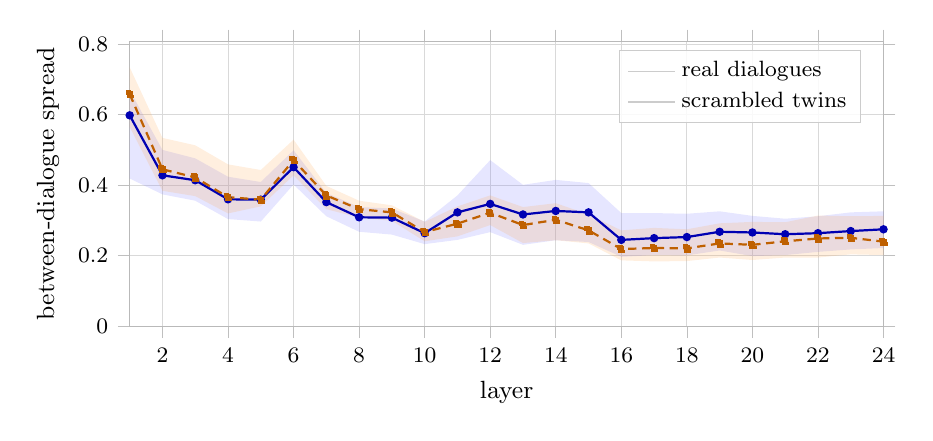
\begin{tikzpicture}
\begin{axis}[width=0.92\linewidth,height=5.2cm,xlabel={layer},ylabel={between-dialogue spread},ymin=0, xmin=1,xmax=24,grid=both,grid style={line width=.2pt,draw=gray!18},major grid style={line width=.3pt,draw=gray!30},tick align=outside,tick style={gray!50},axis line style={gray!55},legend style={font=\footnotesize,draw=gray!40,fill=white,fill opacity=0.85,text opacity=1},legend cell align=left,legend pos=north east,label style={font=\small},tick label style={font=\footnotesize}]
\addplot[draw=none,name path=lor] coordinates {(1,0.419) (2,0.374) (3,0.356) (4,0.304) (5,0.297) (6,0.402) (7,0.312) (8,0.268) (9,0.260) (10,0.233) (11,0.245) (12,0.267) (13,0.231) (14,0.244) (15,0.239) (16,0.197) (17,0.202) (18,0.201) (19,0.215) (20,0.199) (21,0.202) (22,0.211) (23,0.218) (24,0.222)};
\addplot[draw=none,name path=hir] coordinates {(1,0.669) (2,0.500) (3,0.476) (4,0.424) (5,0.409) (6,0.499) (7,0.378) (8,0.338) (9,0.334) (10,0.297) (11,0.371) (12,0.471) (13,0.401) (14,0.415) (15,0.406) (16,0.321) (17,0.321) (18,0.319) (19,0.326) (20,0.313) (21,0.305) (22,0.312) (23,0.323) (24,0.326)};
\addplot[blue!55,opacity=0.18,forget plot] fill between[of=lor and hir];
\addplot[draw=none,name path=los] coordinates {(1,0.565) (2,0.384) (3,0.369) (4,0.320) (5,0.340) (6,0.428) (7,0.332) (8,0.308) (9,0.299) (10,0.241) (11,0.255) (12,0.287) (13,0.236) (14,0.244) (15,0.235) (16,0.187) (17,0.184) (18,0.185) (19,0.195) (20,0.188) (21,0.195) (22,0.195) (23,0.204) (24,0.202)};
\addplot[draw=none,name path=his] coordinates {(1,0.734) (2,0.534) (3,0.513) (4,0.459) (5,0.443) (6,0.529) (7,0.398) (8,0.356) (9,0.343) (10,0.296) (11,0.340) (12,0.371) (13,0.338) (14,0.349) (15,0.317) (16,0.272) (17,0.279) (18,0.275) (19,0.292) (20,0.296) (21,0.295) (22,0.314) (23,0.312) (24,0.313)};
\addplot[orange!70,opacity=0.18,forget plot] fill between[of=los and his];
\addplot[blue!70!black,thick,mark=*,mark size=1.1pt] coordinates {(1,0.598) (2,0.428) (3,0.414) (4,0.360) (5,0.359) (6,0.451) (7,0.352) (8,0.309) (9,0.308) (10,0.264) (11,0.323) (12,0.347) (13,0.317) (14,0.327) (15,0.323) (16,0.245) (17,0.250) (18,0.253) (19,0.268) (20,0.266) (21,0.261) (22,0.264) (23,0.270) (24,0.275)};
\addlegendentry{real dialogues}
\addplot[orange!75!black,thick,densely dashed,mark=square*,mark size=1.1pt] coordinates {(1,0.658) (2,0.445) (3,0.422) (4,0.366) (5,0.359) (6,0.471) (7,0.371) (8,0.332) (9,0.323) (10,0.267) (11,0.291) (12,0.322) (13,0.287) (14,0.302) (15,0.272) (16,0.219) (17,0.222) (18,0.221) (19,0.235) (20,0.231) (21,0.241) (22,0.249) (23,0.251) (24,0.240)};
\addlegendentry{scrambled twins}
\end{axis}
\end{tikzpicture}
\caption{Controlled result ($n{=}12$ dialogues, dialogue-level 95\% CIs). Real (blue) and
scrambled-twin (orange) between-dialogue spread bands overlap at every layer: coherent
content adds nothing detectable beyond the length/topic that the scrambled twin already
matches. Compare to the $n{=}3$ placebo (Figure~\ref{fig:placebo}), which appeared
positive.}
\label{fig:scaled}
\end{figure}

\begin{figure}[t]
\centering
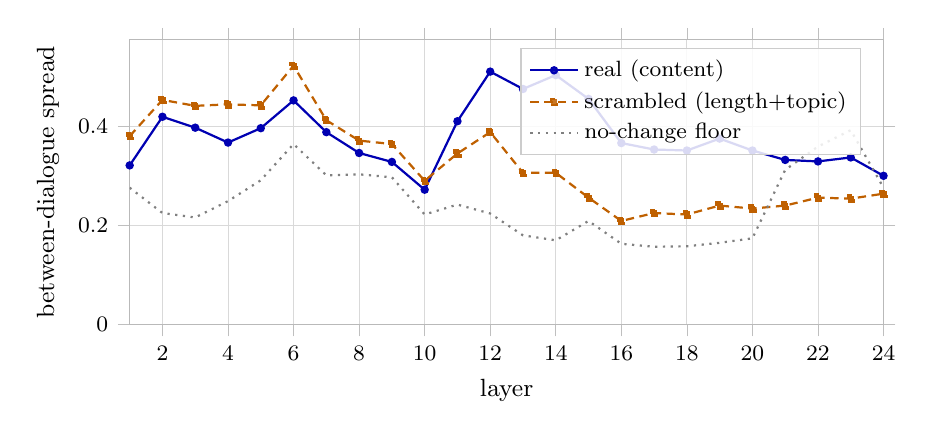
\begin{tikzpicture}
\begin{axis}[width=0.92\linewidth,height=5.2cm,xlabel={layer},ylabel={between-dialogue spread},ymin=0, xmin=1,xmax=24,grid=both,grid style={line width=.2pt,draw=gray!18},major grid style={line width=.3pt,draw=gray!30},tick align=outside,tick style={gray!50},axis line style={gray!55},legend style={font=\footnotesize,draw=gray!40,fill=white,fill opacity=0.85,text opacity=1},legend cell align=left,legend pos=north east,label style={font=\small},tick label style={font=\footnotesize}]
\addplot[blue!70!black,thick,mark=*,mark size=1.1pt] coordinates {(1,0.321) (2,0.419) (3,0.397) (4,0.367) (5,0.396) (6,0.452) (7,0.388) (8,0.346) (9,0.328) (10,0.272) (11,0.410) (12,0.510) (13,0.475) (14,0.503) (15,0.455) (16,0.366) (17,0.353) (18,0.351) (19,0.375) (20,0.351) (21,0.332) (22,0.329) (23,0.337) (24,0.300)};
\addlegendentry{real (content)}
\addplot[orange!75!black,thick,densely dashed,mark=square*,mark size=1.1pt] coordinates {(1,0.380) (2,0.453) (3,0.441) (4,0.444) (5,0.442) (6,0.522) (7,0.412) (8,0.371) (9,0.364) (10,0.290) (11,0.345) (12,0.388) (13,0.306) (14,0.306) (15,0.256) (16,0.209) (17,0.225) (18,0.222) (19,0.240) (20,0.234) (21,0.240) (22,0.256) (23,0.254) (24,0.264)};
\addlegendentry{scrambled (length+topic)}
\addplot[gray,dotted,thick] coordinates {(1,0.276) (2,0.225) (3,0.216) (4,0.249) (5,0.291) (6,0.364) (7,0.301) (8,0.303) (9,0.297) (10,0.222) (11,0.242) (12,0.224) (13,0.180) (14,0.170) (15,0.209) (16,0.163) (17,0.157) (18,0.158) (19,0.165) (20,0.174) (21,0.312) (22,0.359) (23,0.392) (24,0.276)};
\addlegendentry{no-change floor}
\end{axis}
\end{tikzpicture}
\caption{The $n{=}3$ placebo that the controlled result overturns. Early layers (1--10):
scrambled $\geq$ real (a length/lexical artifact). Mid-late layers (11--21): real $>$
scrambled, which \emph{looked} like a content effect but, lacking a dialogue-level CI,
was a small-sample artifact (Figure~\ref{fig:scaled}).}
\label{fig:placebo}
\end{figure}

\begin{figure}[t]
\centering
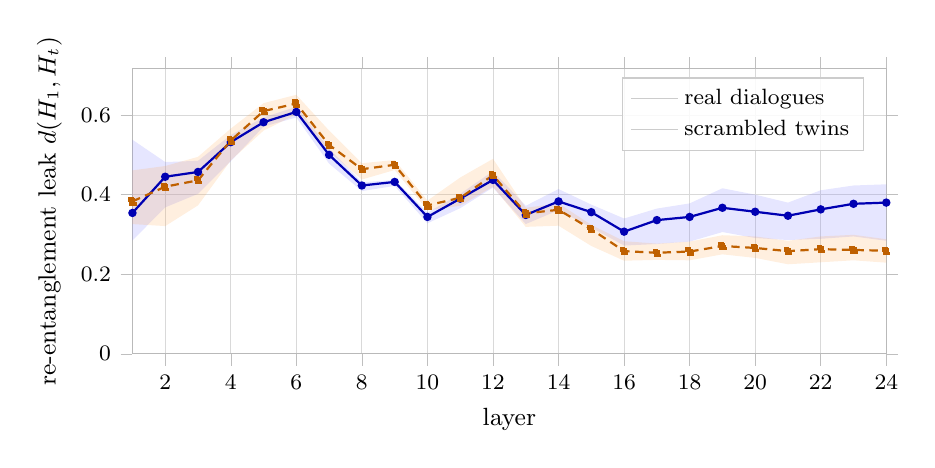
\begin{tikzpicture}
\begin{axis}[width=0.92\linewidth,height=5.2cm,xlabel={layer},ylabel={re-entanglement leak $d(H_1,H_t)$},ymin=0, xmin=1,xmax=24,grid=both,grid style={line width=.2pt,draw=gray!18},major grid style={line width=.3pt,draw=gray!30},tick align=outside,tick style={gray!50},axis line style={gray!55},legend style={font=\footnotesize,draw=gray!40,fill=white,fill opacity=0.85,text opacity=1},legend cell align=left,legend pos=north east,label style={font=\small},tick label style={font=\footnotesize}]
\addplot[draw=none,name path=lor] coordinates {(1,0.285) (2,0.368) (3,0.402) (4,0.484) (5,0.571) (6,0.594) (7,0.478) (8,0.409) (9,0.422) (10,0.328) (11,0.366) (12,0.418) (13,0.326) (14,0.361) (15,0.317) (16,0.272) (17,0.276) (18,0.282) (19,0.306) (20,0.291) (21,0.286) (22,0.289) (23,0.295) (24,0.284)};
\addplot[draw=none,name path=hir] coordinates {(1,0.538) (2,0.482) (3,0.485) (4,0.550) (5,0.594) (6,0.621) (7,0.516) (8,0.431) (9,0.437) (10,0.355) (11,0.402) (12,0.459) (13,0.372) (14,0.414) (15,0.375) (16,0.340) (17,0.365) (18,0.378) (19,0.416) (20,0.400) (21,0.380) (22,0.411) (23,0.423) (24,0.426)};
\addplot[blue!55,opacity=0.18,forget plot] fill between[of=lor and hir];
\addplot[draw=none,name path=los] coordinates {(1,0.326) (2,0.321) (3,0.373) (4,0.486) (5,0.561) (6,0.602) (7,0.508) (8,0.438) (9,0.462) (10,0.361) (11,0.372) (12,0.420) (13,0.319) (14,0.322) (15,0.271) (16,0.234) (17,0.236) (18,0.235) (19,0.250) (20,0.241) (21,0.225) (22,0.230) (23,0.235) (24,0.229)};
\addplot[draw=none,name path=his] coordinates {(1,0.461) (2,0.472) (3,0.495) (4,0.566) (5,0.630) (6,0.651) (7,0.561) (8,0.479) (9,0.487) (10,0.385) (11,0.443) (12,0.490) (13,0.367) (14,0.378) (15,0.324) (16,0.283) (17,0.277) (18,0.282) (19,0.298) (20,0.295) (21,0.284) (22,0.295) (23,0.299) (24,0.288)};
\addplot[orange!70,opacity=0.18,forget plot] fill between[of=los and his];
\addplot[blue!70!black,thick,mark=*,mark size=1.1pt] coordinates {(1,0.354) (2,0.445) (3,0.457) (4,0.532) (5,0.582) (6,0.608) (7,0.500) (8,0.423) (9,0.432) (10,0.344) (11,0.390) (12,0.437) (13,0.349) (14,0.383) (15,0.356) (16,0.307) (17,0.336) (18,0.344) (19,0.367) (20,0.357) (21,0.347) (22,0.363) (23,0.377) (24,0.380)};
\addlegendentry{real dialogues}
\addplot[orange!75!black,thick,densely dashed,mark=square*,mark size=1.1pt] coordinates {(1,0.383) (2,0.420) (3,0.436) (4,0.536) (5,0.610) (6,0.629) (7,0.525) (8,0.464) (9,0.475) (10,0.373) (11,0.392) (12,0.449) (13,0.353) (14,0.362) (15,0.313) (16,0.258) (17,0.254) (18,0.257) (19,0.271) (20,0.266) (21,0.258) (22,0.263) (23,0.261) (24,0.259)};
\addlegendentry{scrambled twins}
\end{axis}
\end{tikzpicture}
\caption{The static disentangling projector (fit at turn 1) re-entangles substantially by
turn 4 (leak $d(H_1,H_4)$, blue), but its length/topic-matched scrambled twin (orange) leaks
just as much: the static baseline's apparent failure is a length/topic artifact, not
content-driven, so a content-conditional projector would not fix it.}
\label{fig:static}
\end{figure}

We report results in five movements. We first validate the estimator and decision rule
against analytic ground truth (\S\ref{sec:res-synth}), then fix the operating point with a
power analysis (\S\ref{sec:res-power}). We then walk the rigor cascade, three intuitive
positive measurements each overturned by the next control (\S\ref{sec:res-cascade}), before
presenting the controlled result and its cross-model and SAE-feature-space replications
(\S\ref{sec:res-controlled}). Finally we fit the static disentangling projector these methods
would replace and show its apparent failure is itself a confound (\S\ref{sec:res-static}).
Every number below is from a run on the released code; the synthetic checks of
\S\ref{sec:res-synth} require no model and reproduce anywhere. Throughout, the
pre-registered decision rule is: a layer is content-conditional iff the real
between-dialogue spread's $95\%$ CI lower bound exceeds the scrambled-twin spread's $95\%$ CI
upper bound, and the verdict is \textsc{content\_conditional} iff a contiguous band of
$\geq 3$ such layers exists.

\subsection{Synthetic validation: the estimator recovers known geometry}
\label{sec:res-synth}

Before touching a model we confirm that the pipeline measures what it claims to. We build
paired activations whose contrast subspace is an analytically controlled object and check
that the estimator and the decision rule behave correctly in three regimes
(Table~\ref{tab:synth}). With a known $15^\circ$/turn rotation injected into the contrast
subspace, the noise-corrected chordal drift is $0.144$ against the analytic value $0.149$, and the decision rule fires positive. With a static (zero-rotation)
subspace the measured drift collapses to the bootstrap noise floor and the rule correctly
returns negative, the property that protects against calling an under-powered run a real
effect. The principal-angle routine returns $0$ for identical planes and $\pi/2$ for
orthogonal ones, confirming the gauge-invariant geometry is implemented correctly. The same
code path is used for every real run below, so a real verdict reflects the data and not a
code artifact.

\begin{table}[t]
\centering
\small
\begin{tabular}{@{}llll@{}}
\toprule
Ground-truth construction & Quantity & Measured & Expected / verdict \\
\midrule
$15^\circ$/turn injected rotation & noise-corrected drift & $0.144$ & $0.149$ (analytic) \\
static (zero-rotation) subspace & drift & at bootstrap floor & negative (correct) \\
identical planes & principal angle & $0$ & $0$ \\
orthogonal planes & principal angle & $\pi/2$ & $\pi/2$ \\
\bottomrule
\end{tabular}
\caption{Synthetic validation against analytic ground truth (no model, no network). The
estimator recovers an injected rotation accurately ($0.144$ vs.\ $0.149$), returns the bootstrap floor (a
correct negative) for a static subspace, and passes the principal-angle sanity checks.}
\label{tab:synth}
\end{table}

\subsection{Power analysis: rank-1 and $\geq 96$ probes}
\label{sec:res-power}

Subspace estimation in $d\!\approx\!10^3$ activation space is noisy, and the bootstrap noise
floor (the drift between two resamples of the \emph{same} subspace) sets the smallest effect
the protocol can resolve. On \texttt{Qwen2.5-0.5B-Instruct} (raw activations, rank-1) the
$95\%$ floor falls from $0.49$ at $16$ probes to $0.22$ at $96$ probes, scaling as
$\approx 1/\sqrt{n_{\text{probes}}}$ (Table~\ref{tab:power}). Higher-rank subspaces are not
usable at these sample sizes: a rank-2 or rank-3 fit from a few dozen probes returns a floor
of $\approx 0.7$, meaning two estimates of the \emph{same} subspace are nearly orthogonal, so
the recovered directions are noise. We therefore operate at rank-1 with $\geq 96$ probe pairs
per side, and we report the floor alongside every drift so that a null is never mistaken for
an under-powered run.

Power is summarized in Table~\ref{tab:power} (Section~\ref{sec:power}).

\subsection{The rigor cascade: three positive measurements, each overturned}
\label{sec:res-cascade}\label{sec:cascade}

We arrived at the controlled result through a sequence of measurements of increasing rigor,
each of which caught a confound in the previous one (Table~\ref{tab:cascade}). We present the
cascade in full because it is itself a contribution: it shows concretely how intuitive
measurements of representational drift produce false positives, and which control removes each.

\begin{table}[t]
\centering
\small
\begin{tabular}{@{}llll@{}}
\toprule
Step & Measurement & Headline & Overturned by \\
\midrule
1 & consecutive drift, 32 probes, one layer & inconclusive (under-powered) & noise floor too high \\
2 & cumulative drift from turn 0 & \textcolor{red}{positive} & turn-0 onset confound \\
3 & spread vs same-context floor & \textcolor{red}{positive} (21 layers) & floor carries no length variance \\
4 & scrambled placebo, $n{=}3$ dialogues & \textcolor{red}{positive} (layers 11--21) & $n{=}3$, no CI; one outlier dialogue \\
5 & \textbf{scrambled, $n{=}12$, dialogue-level CI} & \textbf{negative} & (the controlled result) \\
\bottomrule
\end{tabular}
\caption{Each row's headline was overturned by the next control. Steps 2--4 are \emph{false
positives} produced by intuitive but confounded measurements; step 5 is the controlled result
reported in \S\ref{sec:res-controlled}.}
\label{tab:cascade}
\end{table}

\paragraph{Step 1 (under-power).} A consecutive-turn drift with only $32$ probes at a single
layer is inconclusive: the noise floor at $32$ probes ($0.31$, Table~\ref{tab:power}) is
comparable to any motion present, so nothing can be concluded. This is why power must be fixed
first.

\paragraph{Step 2 (no-context onset, a false positive).} Measuring cumulative drift from turn
$0$ produces a large, apparently positive signal. The tell is that the between-dialogue spread
($\approx 0.37$) is far below the turn-$0$ displacement ($\approx 0.88$): almost all of the
motion is the generic bare-probe$\to$probe-in-context jump, which is shared across dialogues
and is not content-conditional. Baselining at turn $1$ and measuring $d(U_1,U_t)$ removes it.

\paragraph{Step 3 (same-context floor, a false positive over 21 layers).} Comparing the
between-dialogue spread against a same-context resampling floor looks positive at $21$ layers,
but this comparison is near-tautological. The floor resamples probes within one fixed context
and therefore contains zero between-dialogue length, topic, and position variance, while the
spread contains all of it. Empirically the between-dialogue spread grew monotonically with
turn index in lockstep with the per-turn token-length gap, which widened from $3$ to $20$
tokens across turns ($\approx 12\%$ at the turn where the spread is measured): the signature
of a length artifact, not of content.

\paragraph{Step 4 (small-sample placebo, a false positive at layers 11--21).} Introducing the
scrambled-twin null with $n{=}3$ dialogues appears to rescue a content effect at the
mid-to-late layers (layers $11$--$21$, real $>$ scrambled; Figure~\ref{fig:placebo}). But this
is a point estimate with no confidence interval, and its median rests on a single
topically-divergent dialogue. Resampling at the dialogue level dissolves it.

\paragraph{Step 5 (the controlled result).} With $n{=}12$ dialogues, the scrambled-twin null,
and a dialogue-level bootstrap CI, the verdict is negative. This is the controlled measurement
we report next.

\subsection{Controlled result and replications}
\label{sec:res-controlled}

\paragraph{Model and data.} We report \texttt{Qwen2.5-0.5B-Instruct} \citep{qwen25}
($896$-dim residual stream, $24$ layers), rank-1 difference-of-means directions, $64$--$96$
probe pairs per side, and $12$ topically diverse $5$-turn dialogues. For the headline test we
take each dialogue's final-turn (full-context) hallucination subspace $H_t$ at every layer,
compute the median pairwise between-dialogue chordal spread, and bracket it with a
dialogue-level bootstrap $95\%$ CI, against the length- and topic-matched scrambled-twin null.

\paragraph{The hallucination subspace is not content-conditional on this model.} The apparent
content-conditionality does not survive (Figure~\ref{fig:scaled}, Table~\ref{tab:qwen05}). At
\emph{every} layer the real-dialogue spread CI overlaps the scrambled-twin spread CI: at layer
$12$, real $0.347$ $[0.27,0.47]$ versus scrambled $0.322$ $[0.29,0.37]$; at layer $15$, real
$0.323$ $[0.24,0.41]$ versus scrambled $0.272$ $[0.24,0.32]$. A small, consistent,
non-significant trend remains at the mid-to-late layers (real slightly above scrambled), but no
layer satisfies the decision rule (real CI lower bound $>$ scrambled CI upper bound), so no
contiguous band exists and the verdict is \textsc{not\_content\_conditional}. Scrambled twins,
which hold token length, position, and lexical topic fixed while destroying coherent dialogue
meaning, move the hallucination subspace as much as the real dialogues do. The between-dialogue
movement is therefore attributable to length and topic, not to coherent dialogue content.

\begin{table}[t]
\centering
\small
\begin{tabular}{@{}lccc@{}}
\toprule
Layer & Real spread $[95\%\ \text{CI}]$ & Scrambled spread $[95\%\ \text{CI}]$ & Clears rule? \\
\midrule
$12$ & $0.347$ $[0.27,0.47]$ & $0.322$ $[0.29,0.37]$ & no \\
$15$ & $0.323$ $[0.24,0.41]$ & $0.272$ $[0.24,0.32]$ & no \\
\bottomrule
\end{tabular}
\caption{Controlled result on \texttt{Qwen2.5-0.5B-Instruct} (raw activations, $24$ layers,
$n{=}12$ dialogues, rank-1, dialogue-level bootstrap). Representative mid-late layers: real and
scrambled-twin CIs overlap, no layer clears the decision rule, and no $\geq 3$-contiguous band
forms. Verdict: \textsc{not\_content\_conditional}.}
\label{tab:qwen05}
\end{table}

\paragraph{The safety side is worse, not better.} The premise that matters for conditional
\emph{disentanglement} concerns the joint geometry of $S_t$ and $H_t$. On this model the
refusal direction is not cleanly recoverable below the mid layers: two independent estimates of
the same $S$ subspace are near-orthogonal (floor $\approx 1.0$) through roughly the first half
of the network, becoming recoverable only at the later layers. The cross-subspace overlap
$\Omega(S_t,H_t)$ is therefore meaningful only at late layers, where its movement across turns
is small. We thus cannot even measure the entanglement drift that conditional disentanglement
is designed to track, let alone show it is large.

\paragraph{Replication across model scale (Qwen2.5-1.5B).} The same controlled test on
\texttt{Qwen2.5-1.5B-Instruct} ($28$ layers, $n{=}12$, rank-1) returns the same verdict: the
content-conditional band is empty (Table~\ref{tab:qwen15}). At layer $1$, real $0.653$
$[0.56,0.69]$ versus scrambled $0.665$ $[0.57,0.72]$; at the late layers real slightly exceeds
scrambled but the CIs overlap throughout, so no layer clears the rule. The null is therefore
not an artifact of the smallest model.

\begin{table}[t]
\centering
\small
\begin{tabular}{@{}lccc@{}}
\toprule
Layer & Real spread $[95\%\ \text{CI}]$ & Scrambled spread $[95\%\ \text{CI}]$ & Clears rule? \\
\midrule
$1$ & $0.653$ $[0.56,0.69]$ & $0.665$ $[0.57,0.72]$ & no \\
late layers & real slightly $>$ scrambled & CIs overlap throughout & no \\
\bottomrule
\end{tabular}
\caption{Cross-scale replication on \texttt{Qwen2.5-1.5B-Instruct} (raw activations, $28$
layers, $n{=}12$, rank-1). The content-conditional band is empty; verdict
\textsc{not\_content\_conditional}.}
\label{tab:qwen15}
\end{table}

\paragraph{Replication in SAE feature space (GPT-2 small).} Because disentanglement methods
operate on SAE features rather than raw activations, we repeated the controlled test in the
feature space of GPT-2 small using the publicly released residual-stream SAEs at all twelve
layers \citep{cunningham2023sparse, bricken2023monosemanticity}, encoding each contrastive
probe's last-token activation through the frozen SAE and recovering $H_t$ in feature
coordinates. The verdict is unchanged: at no layer does the real between-dialogue spread clear
the scrambled-twin spread, the band is empty, and at the late layers ($7$--$11$), where
abstract features concentrate, the scrambled spread is in fact \emph{larger} than the real
spread (Table~\ref{tab:gpt2sae}). At layer $10$, real $0.515$ $[0.46,0.58]$ versus scrambled
$0.659$ $[0.58,0.80]$; at layer $11$, real $0.541$ $[0.47,0.64]$ versus scrambled $0.668$
$[0.59,0.74]$. The apparent context-dependence is, if anything, \emph{better} explained by
length and lexical content in feature space than in raw space. The null is thus not an artifact
of the activation basis: it holds in the exact representation conditional disentanglement would
use.

\begin{table}[t]
\centering
\small
\begin{tabular}{@{}lccc@{}}
\toprule
Layer & Real spread $[95\%\ \text{CI}]$ & Scrambled spread $[95\%\ \text{CI}]$ & Scrambled $>$ real? \\
\midrule
$10$ & $0.515$ $[0.46,0.58]$ & $0.659$ $[0.58,0.80]$ & yes \\
$11$ & $0.541$ $[0.47,0.64]$ & $0.668$ $[0.59,0.74]$ & yes \\
\bottomrule
\end{tabular}
\caption{SAE-feature-space replication on GPT-2 small (\texttt{gpt2-small-res-jb} residual
SAEs, all $12$ layers, $n{=}12$, rank-1). The band is empty, and at the late layers the
scrambled-twin spread \emph{exceeds} the real spread: length and lexical content explain the
movement at least as well as coherent content. Verdict \textsc{not\_content\_conditional}.}
\label{tab:gpt2sae}
\end{table}

\subsection{Demonstration: the static baseline does not genuinely fail}
\label{sec:res-static}

The premise's operational consequence is that a \emph{static} disentangling projector, fit
once, should fail at later turns, which is what motivates replacing it with a conditional one.
We test this directly on \texttt{Qwen2.5-0.5B-Instruct} ($n{=}12$). The static projector built
at turn $1$ nulls the hallucination subspace $H_1$; its residual re-entanglement leak at turn
$t$, the fraction of $H_t$ the frozen projector fails to remove, is exactly $d(H_1,H_t)\in[0,1]$,
while a conditional projector rebuilt at turn $t$ has leak $0$ by construction. Naively the
static projector looks broken: its leak by turn $4$ is large, $0.3$--$0.6$ across layers
(Figure~\ref{fig:static}). But the length- and topic-matched scrambled twins leak \emph{just as
much} (Table~\ref{tab:static}): at layer $8$, real $0.423$ $[0.41,0.43]$ versus scrambled
$0.464$ $[0.44,0.48]$; at layer $12$, real $0.437$ versus scrambled $0.449$. Only $3$ of $25$
layers (all late: $18$, $19$, $21$) show real leak exceeding scrambled at the dialogue-level
$95\%$ level, and they are not contiguous, below our pre-registered $\geq 3$-contiguous-layer
rule and near the $\approx 1.25$ layers expected by chance. We report this weak, non-robust
late-layer elevation rather than hide it. The verdict is \textsc{static\_failure\_is\_confound}:
for this behavior and model, a static projector's degradation across turns is confound-explained,
so a content-conditional projector would not fix it and the conditional machinery addresses a
confound rather than a real non-stationarity.

\begin{table}[t]
\centering
\small
\begin{tabular}{@{}lccc@{}}
\toprule
Layer & Real leak $d(H_1,H_t)$ $[95\%\ \text{CI}]$ & Scrambled leak $[95\%\ \text{CI}]$ & Real $>$ scrambled? \\
\midrule
$8$ & $0.423$ $[0.41,0.43]$ & $0.464$ $[0.44,0.48]$ & no \\
$12$ & $0.437$ & $0.449$ & no \\
\midrule
\multicolumn{4}{@{}l}{Only $3/25$ layers (late: $18,19,21$) cross the dialogue-level bar; \emph{not} contiguous ($\geq 3$ rule unmet; chance $\approx 1.25$).} \\
\bottomrule
\end{tabular}
\caption{Static-projector demonstration on \texttt{Qwen2.5-0.5B-Instruct} ($n{=}12$). The
static projector's apparent across-turn re-entanglement is matched by its length/topic
scrambled twin, so it does not genuinely fail. Verdict \textsc{static\_failure\_is\_confound}.}
\label{tab:static}
\end{table}

\paragraph{Summary across settings.} Every configuration tested under the full protocol
(\texttt{Qwen2.5-0.5B-Instruct} and \texttt{Qwen2.5-1.5B-Instruct} in raw activation space, and
GPT-2 small in SAE feature space) returns \textsc{not\_content\_conditional}, and the
static-projector demonstration returns \textsc{static\_failure\_is\_confound}. On the
instruction-tuned and GPT-2 models we evaluate, in raw and SAE feature space, the apparent
context-conditionality of the hallucination subspace is statistically indistinguishable from a
length and topic artifact.

% =====================================================================
% REPRODUCIBILITY APPENDIX
% =====================================================================


\section{Discussion, Scope, and Limitations}
\label{sec:limits}

\paragraph{What this does and does not establish.} It establishes that, for the model and
construction tested, three intuitive measurements of context-conditionality are
confounded, and that the controlled measurement returns a null. It does \emph{not}
establish that the premise is universally false. The most important open cells, which we
are running and which any method paper relying on the premise should report, are:
\textbf{(a)} SAE feature space on an \emph{instruction-tuned} model (we have shown the
null replicates in GPT-2 SAE space for the hallucination subspace; the safety side needs a
chat model with released SAEs, e.g.\ Gemma~2 with Gemma Scope, \citealp{lieberum2024gemmascope});
\textbf{(b)} larger instruction-tuned models, where the
refusal direction is recoverable at more layers and the safety side becomes testable;
\textbf{(c)} a mixture-of-experts model, for the per-expert variant of the premise;
\textbf{(d)} higher-rank subspaces; and \textbf{(e)} a direct test of mis-specification,
fitting a static disentangling projector and measuring whether it re-entangles at later
turns. Our protocol ports to all five with only a change of backend.

\paragraph{Residual confounds in the control.} The scrambled twin holds token length and
topic but conflates coherent ``dialogue content'' with ``epistemic state''; a fully
within-topic content manipulation would separate these. Word-shuffling may also partially
degrade topic extraction; this would, if anything, bias toward a (spurious) positive,
which we do not observe.

\paragraph{Implication.} The negative result is not an indictment of conditional steering
or disentanglement; it is a request that such methods measure, with controls, the premise
they assume. A static intervention is mis-specified only if the geometry it freezes
actually moves with context beyond length and topic. On the present evidence, the cheap
and decisive thing is to run the controlled measurement first.

\section{Lessons and Actionable Recommendations}
\label{sec:lessons}

The point of this study is not the single null but the transferable lessons that produced
it; we state them as recommendations for two audiences.

\paragraph{For anyone measuring whether a manipulation changes a representation}
(context, in-context examples, a steering edit, a fine-tune), the following four controls
flip conclusions in practice and should be standard:
\begin{enumerate}
\item \textbf{Use a matched-null, not a same-condition resampling floor.} A bootstrap over
probes at a fixed condition contains none of the between-condition variance (length, position,
topic) that the test statistic carries, so ``effect $>$ floor'' is near-tautological. Build a
null that matches the nuisance variables and differs only in the variable of interest (here,
length/topic-matched scrambled twins). This single change converted our headline from
positive to null.
\item \textbf{Measure with a gauge-invariant quantity.} Subspaces are recovered up to an
arbitrary basis; a basis-dependent ``drift'' conflates estimator gauge with real movement.
Use principal-angle/chordal distances.
\item \textbf{Bootstrap over the unit of generalization, not the convenient one.} A
confidence interval over probes says nothing about generalization across dialogues; resample
the dialogues. Our mid-layer ``effect'' was significant over probes and vanished over
dialogues ($n{=}3 \to n{=}12$).
\item \textbf{Baseline away trivial transitions.} The no-context$\to$context jump is large,
shared, and uninteresting; measure drift relative to the first in-context turn, and report the
onset separately.
\end{enumerate}

\paragraph{For designers of conditional alignment methods} (conditional steering, conditional
disentanglement): a conditional intervention is justified only if the geometry it conditions on
\emph{moves} with context beyond nuisance confounds, and if a static baseline \emph{fails}. We
recommend reporting, as a precondition, (i) the controlled context-conditionality measurement
above, in the feature space the method uses, and (ii) a static-projector baseline tested for
content-driven re-entanglement. We carried out exactly this test (\S\ref{sec:main},
Figure~\ref{fig:static}): the static projector's across-turn leak is fully matched by the
length/topic placebo, so it does not genuinely fail. On the present evidence the conditional
machinery, for the behaviors and models studied, addresses a confound rather than a real
non-stationarity. We do not claim this generalizes to all settings; we claim that without this
controlled check a method cannot tell the two apart, and the check is cheap.

\paragraph{A reusable checklist.} The released harness packages the above as a drop-in test:
a gauge-invariant drift metric, a scrambled-twin null, dialogue-level bootstrap CIs, a power
curve, and a synthetic ground-truth validation, with a single backend swap between raw
activations and SAE features. The intended use is pre-registration: run it, report the
controlled measurement and the power, and only then build (or not).

\section{Conclusion}

We asked whether dialogue context rotates the safety and hallucination subspaces of an LLM,
the premise underlying conditional disentanglement. The obvious measurements say yes; each
is a confound. Under a length/topic-matched, dialogue-level-bootstrapped protocol the
effect is within noise on the model tested, and the safety subspace is not recoverable
where the premise would need to hold. We release the protocol and the full rigor cascade so
that representational-drift claims, positive or negative, can be vetted before they are
built upon.

\paragraph{Reproducibility.} All code, probe banks, dialogues, cached activations, and the
synthetic ground-truth validation are released; every figure and number is regenerated by
the released scripts.

\appendix

\section{Synthetic Validation Details}
\label{app:synth}

The synthetic test (Table~\ref{tab:synth}) runs with no model and no network and reproduces on
any machine, so it isolates the estimator and decision rule from any property of a particular
language model. We construct paired activations whose contrast subspace is an analytically
known object, then check four properties.

\paragraph{Construction.} For each turn we draw class-conditional activation clouds whose
difference-of-means defines a rank-$k$ ground-truth subspace with a prescribed orientation.
Two ground-truth trajectories are used: a \emph{static} subspace whose orientation is fixed
across turns, and a \emph{rotating} subspace whose orientation advances by a fixed
$15^\circ$ per turn. Estimation noise is controlled by the number of probe pairs, matching the
power regime used on real data (\S\ref{sec:res-power}).

\paragraph{What it confirms.} (i) At high SNR the estimator recovers the injected subspace.
(ii) The static trajectory returns measured drift at the bootstrap noise floor, and the
decision rule returns negative, the property that prevents a low-power run from being read as a
positive. (iii) The $15^\circ$/turn rotation is recovered as noise-corrected chordal drift
$0.144$ against the analytic $0.149$, clears the floor, and the rule
returns positive; a cross-subspace overlap with a known time-varying relative angle is tracked
over the same trajectory. (iv) Principal-angle sanity: identical planes return $0$, orthogonal
planes return $\pi/2$. Because the identical code path is used on real data, a verdict on a real
model reflects the data rather than a code artifact.

\section{Evaluation Matrix: Done and Pending}
\label{app:matrix}

Table~\ref{tab:matrix} records the evaluation matrix. The acceptance risk for a scoped negative
is not novelty but breadth, the objection that the effect was missed because of the wrong model,
space, or rank; we therefore enumerate the cells that close that objection and mark each as done
or pending, with the released harness producing the statistic for both. The single most
important pending cell is the safety subspace in SAE feature space on an instruction-tuned chat
model (e.g.\ Gemma~2 with Gemma Scope, \citealp{lieberum2024gemmascope}). It is supported by the
released harness but is pending larger compute: a \texttt{transformer\_lens} plus Gemma-2 load
issue prevented it on the available T4, and it is expected to complete on an A100-class GPU. We
mark it pending rather than report it.

\begin{table}[t]
\centering
\small
\begin{tabular}{@{}llc@{}}
\toprule
Cell & Objection it closes & Status \\
\midrule
Qwen2.5-0.5B-Instruct, raw acts, rank-1 & baseline & done \\
Qwen2.5-1.5B-Instruct, raw acts, rank-1 & ``only the smallest model'' & done \\
GPT-2 small, SAE feature space, rank-1 & ``raw acts aren't where methods operate'' & done \\
static-projector demonstration (Qwen2.5-0.5B) & ``you never tested the actual claim'' & done \\
safety subspace in SAE space, instruction-tuned (Gemma-2 + Gemma Scope) & SAE safety side on a chat model & pending (A100) \\
mixture-of-experts model (per-expert premise) & per-expert variant of the premise & pending \\
rank-$2$/$3$ subspaces & ``rank-1 is too crude'' & pending (needs hundreds of probes) \\
within-topic content control & ``topic conflated with content'' & pending \\
behavioral (generation-time) static-projector test & generation-time mis-specification & pending (future work) \\
\bottomrule
\end{tabular}
\caption{Evaluation matrix. Raw-activation replication across two model scales and the SAE
feature-space replication (GPT-2) are complete, as is the static-projector demonstration. The
instruction-tuned SAE cell for the safety subspace is supported by the released harness but
pending a larger GPU. The protocol ports to every pending cell with only a backend swap.}
\label{tab:matrix}
\end{table}

\section{Probe-Bank Construction}
\label{app:probes}

\paragraph{Contrastive pairs.} Subspaces are recovered by contrast, following standard practice
in the probing and steering literature. The \emph{hallucination/epistemic} subspace $H_t$ is the
rank-1 difference-of-means direction between answerable real-entity questions and surface-matched
unanswerable fictional-entity questions, following the knowledge-awareness construction of
\citet{ferrando2025entity}. The \emph{safety} subspace $S_t$ is the analogous contrast between
harmful requests and surface-matched harmless requests, the refusal direction of
\citet{arditi2024refusal}. Pairs are surface-matched so that the recovered direction isolates the
epistemic or safety contrast rather than lexical or syntactic differences.

\paragraph{Fixed probes, varying context.} At dialogue turn $t$ we prepend the running
conversation (the first $t$ user turns, each followed by a fixed neutral assistant reply) and
append the contrastive probe bank as the next user turn, reading the last-token residual
activation at each layer. The probes are held fixed and only the prepended context varies, so any
movement in the recovered $U_t$ is attributable to context.

\paragraph{Power-driven sizing.} The power analysis (\S\ref{sec:res-power}) requires $\geq 96$
probe pairs per side at rank-1; we use $40$--$96$ pairs per side in the reported runs. The
deliberately small banks used for laptop development are not large enough for a publishable
verdict, which is precisely why the floor is reported with every drift.

\paragraph{Scrambled-twin null.} The length- and topic-matched null is generated by
word-shuffling each user turn. This preserves the exact token multiset (and hence length, topic,
and lexicon) while destroying coherent meaning, so genuine content-conditionality requires the
real subspace to move more than its scrambled twin. As noted in the scope discussion, the
scrambled twin holds topic fixed but conflates coherent dialogue content with epistemic state; a
fully within-topic manipulation (a pending cell) would separate the two.

\section{Reproducibility Statement}
\label{app:repro}

All code, probe banks, dialogue scripts, cached activations, and the synthetic ground-truth
validation are released in a public repository. Every figure and number in this paper, including
the synthetic validation (Table~\ref{tab:synth}), the power curve (Table~\ref{tab:power}), the
rigor cascade (Table~\ref{tab:cascade}), the controlled result and its cross-model and
SAE-feature-space replications (Tables~\ref{tab:qwen05}--\ref{tab:gpt2sae}), the static-projector
demonstration (Table~\ref{tab:static}), and Figures~\ref{fig:scaled}, \ref{fig:placebo}, and
\ref{fig:static}, is regenerated by the released scripts.

\paragraph{Pipeline.} The estimator and decision rule are validated with a model-free synthetic
test that reproduces anywhere. Activation extraction reads the last-token residual stream at each
layer; the SAE-feature-space backend passes that activation through the frozen released SAE
encoder and runs the identical contrast-and-drift pipeline on the feature vector, so the only
change between the raw and SAE settings is a backend swap. Drift is computed as the
gauge-invariant chordal distance with dialogue-level bootstrap confidence intervals, and the
pre-registered decision rule (real CI lower bound $>$ scrambled CI upper bound over a
$\geq 3$-contiguous-layer band) is applied uniformly across all settings.

\paragraph{Determinism and scope.} Random seeds for the bootstrap and for synthetic data
generation are fixed, so the reported intervals reproduce. The released harness packages the
gauge-invariant drift metric, the scrambled-twin null, dialogue-level bootstrap CIs, the power
curve, and the synthetic validation as a drop-in test with a single backend swap between raw
activations and SAE features, so that a representational-drift claim, positive or negative, can be
vetted before it is built upon. All results are scoped to the models and feature spaces evaluated
here, \texttt{Qwen2.5-0.5B-Instruct} and \texttt{Qwen2.5-1.5B-Instruct} in raw activation space and
GPT-2 small in SAE feature space; we do not claim the verdict generalizes beyond them.

\bibliography{refs}
\bibliographystyle{tmlr}

\end{document}
